% Diese Zeile bitte -nicht- aendern.
\documentclass[course=erap]{aspdoc}

%%%%%%%%%%%%%%%%%%%%%%%%%%%%%%%%%
%% TODO: Ersetzen Sie in den folgenden Zeilen die entsprechenden -Texte-
%% mit den richtigen Werten.
\newcommand{\theGroup}{134} % Beispiel: 42
\newcommand{\theNumber}{A319} % Beispiel: A123
\author{Chen Yang \and Qichen Liu \and Tanmay Amarendra Deshpande}
\date{Sommersemester 2023} % Beispiel: Wintersemester 2019/20
%%%%%%%%%%%%%%%%%%%%%%%%%%%%%%%%%

% Diese Zeile bitte -nicht- aendern.
\title{Gruppe \theGroup{} -- Abgabe zu Aufgabe \theNumber}
\usepackage{algorithm}
\usepackage{algpseudocode}
\usepackage{bchart}
\usepackage{tikz}
\usepackage{pgfplots}
\usepackage{amsmath}
\usepackage{mathtools}
\begin{document}
\maketitle

\section{Einleitung}
\subsection{Arithmetik in Zahlensystemen mit komplexer Basis}
Wir kennen die g-adische Schreibweise einer Zahl $A$ als Abfolge von Ziffern $a_i$ mit ihrer Position entsprenchender Wertigkeit gemäß $g$:
\begin{eqnarray}
A = \sum_{i = 0}^{n} a_i \cdot g^i \nonumber
\end{eqnarray}
In der Aufgabe beschäftigen wir uns mit Arithmetik in Zahlensystemen, die auf einer komplexen Basis $g = -1 + i$ mit $i^2 = -1$ basieren.\\
Somit\cite{Penney1965AS} können alle komplexen Zahlen mit ganzen Real- und Imaginärteilen dargestellt werden, und das sogar, wenn man $a_i$ als Elemente der Menge $\{0, 1\}$ festsetzt. \\
Das Letztere bezieht sich auf die übliche binäre Zifferndarstellung in der Informatikwelt. Wir entwerfen daher einen Rechner, der zwischen der üblichen kartesischen Darstellung einer komplexen Zahl $a + bi$ und ihrer Darstellung zur Basis $-1 + i$ konvertieren kann.

\subsection{Aufgabenstellung}
Die Aufgabe lässt sich in die Bereiche Konzeption (theoretisch) und Implementierung (praktisch) aufteilen. Antworten auf konzeptionelle Fragen werden an den passenden Stellen in der Ausarbeitung erscheinen. Für die Implementierung sind die folgenden zwei Signaturen in der Programmiersprache C vorgegeben.


% \begin{lstlisting}[language=C]
% void to_carthesian(unsigned __int128 bm1pi, __int128* real, __int128* imag);
% unsigned __int128 to_bm1pi(__int128 real, __int128 imag);
% \end{lstlisting} 

\begin{lstlisting}[language=C, basicstyle=\small\ttfamily]
void to_carthesian(unsigned __int128 bm1pi, __int128* real, __int128* imag);
unsigned __int128 to_bm1pi(__int128 real, __int128 imag);
\end{lstlisting}
\noindent
Die Funktion \texttt{void to\_carthesian} konvertiert eine komplexe Zahl \texttt{unsigned \_\_int128 bm1pi} zur Basis $-1 + i$ in ihre übliche kartesische Darstellung. Der Realteil wird an die Adresse \texttt{\_\_int128 *real} gespeichert und der Imaginärteil an die Adresse \texttt{\_\_int128 *imag}.\\
Die Funktion \texttt{unsigned \_\_int128 to\_bm1pi} konvertiert die übliche kartesische Darstellung einer komplexen Zahl mit dem Realteil \texttt{\_\_int128 real} und dem Imaginärteil \texttt{\_\_int128 imag} in ihre Darstellung zur Basis $-1 + i$. Das Ergebnis wird als \texttt{unsigned \_\_int128} zurückgegeben.\\
Es ist wichtig anzumerken, dass in der Implementierung nur die vier Grundrechenarten $(+, -, \times, \div)$ erlaubt sind.

\section{Lösungsansatz}
\subsection{Umrechnung von der kartesischen Form in die Basis $-1 + i$\cite{CtoBNaive}} 
Eine Dezimalzahl lässt sich in eine andere Basis konvertieren, indem man die Zahl ständig durch den Wert der neuen Basis dividiert, bis man auf die 0 kommt und bei jedem Divisionsschritt den Rest notiert. Man baut dann die neue Darstellung auf, indem man die Reste der Divisionen in umgekehrter Reihenfolge aneinanderhängt. Als Beispiel rechnen wir die Dezimalzahl 9 in das Binärsystem um. Ergebnis: $9_{10} = 1001_2$.
\begin{center}
    \begin{tabular}{||c|c|c| c||}
    \hline
    Dividend & Divisor & Quotient & Rest\\
    \hline
    9 & 2  & 4  & 1\\
    \hline
    4 & 2  & 2  & 0\\
    \hline
    2 & 2  & 1  & 0\\
    \hline
    1 & 2  & 0  & 1\\
    \hline
    \end{tabular}
\end{center}
Analog lässt sich die Zahl auch in die Basis $-1 + i$ konvertieren. 
Sei die komplexe Zahl in Dezimalsystem $a + bi$ wobei $a$ den Realteil und $b$ den Imaginärteil sind. Nach einer Division durch $-1 + i$ erhalten wir:
$$\frac{a + bi}{-1 + i} = \frac{b-a}{2} - \frac{a + b}{2}\cdot i $$
\textbf{Fall 1: a und b beide gerade bzw. beide ungerade:}\\
Sowohl $b - a$ als auch $a + b$ sind durch 2 teilbar. Daher erhalten wir den Quotienten $\frac{b-a}{2} - \frac{(a + b)i}{2}$ mit einem Rest von 0.\\
\textbf{Fall 2: a gerade und b sind ungerade oder umgekehrt: }\\
Sowohl $b - a$ als auch $a + b$ ungerade. Die Quotienten lassen sich aber wie folgt umformulieren, somit haben wir den Rest von 1 mit dem Quotienten $\frac{b-a +1}{2} - \frac{a + b - 1}{2} \cdot i$
$$\frac{b-a}{2} - \frac{a + b}{2}\cdot i  = \frac{b-a +1}{2} - \frac{a + b - 1}{2} \cdot i -\frac{1 + i}{2}$$
Daraus folgt, dass der Rest entweder 0 oder 1 ist. Somit können komplexe Zahlen als einzelner Bitstring dargestellt werden, anstatt den Real- und Imaginärteil getrennt zu schreiben. Bei jedem Schritt der Division wenden wir die entsprechenden Formeln für den Quotienten an, je nachdem ob beide Teile gerade oder ungerade sind oder unterschiedliche Teilbarkeiten durch 2 aufweisen, und setzen den Rest auf 0 bzw. 1. Der Algorithmus wird beendet, wenn sowohl der Realteil als auch der Imaginärteil 0 sind. Als Beispiel rechnen wir $3 - 2i$ in  Basis $-1 + i$ um:
\begin{align*}
\begin{tabular}{||c|c | c| c| c | c ||}
     \hline
     Dividend (Real) & Dividend(Imag) & Divisor & Quo. (Real) & Quo.(Imag) & Rest\\
     \hline
     3 & -2 & $-1  + i$ & -2 & 0 & 1\\
     \hline
     -2 & 0 & $-1  + i$ & 1 & 1 & 0\\
     \hline
     1 & 1 & $-1  + i$ & 0 & -1 & 0\\
     \hline
     -1 & 0 & $-1  + i$ & 0 & 1 & 1\\
     \hline
     0 & 1 & $-1  + i$ & 1 & 0 & 1\\
     \hline
     1 & 0 & $-1  + i$ & 0 & 0 & 1\\
     \hline
\end{tabular}
\end{align*}
Als Ergebnis lesen wir die Reste in umgekehrter Reihenfolge: $(111001)_{-1 + i}$
\subsubsection{to\_bm1pi\_V1: Naive Implementierung}
Die naive Implementierung übersetzt den Algorithmus aus dem vorherigen Abschnitt \cite{CtoBNaive} in C-Code mithilfe einer while-Schleife. Der Real- und Imaginärteil werden vor der nächsten Iteration gemäß den Formeln aktualisiert, bis beide Teile den Wert 0 erreichen. Das Setzen des Bitstrings (abhängig vom Rest in jeder Iteration) erfolgt durch Verwendung einer Maske, die anfangs den Wert 1 hat und bei jeder Iteration um eine Position nach links verschoben wird. Durch Veroderung (OR) mit dem Bitstring kann die entsprechende Position auf den Wert 1 gesetzt werden.
Die Variable \texttt{shift} zählt, um wie viele Stellen die Maske nach links verschoben wurde. Falls die Maske mehr als 128 Mal verschoben wurde, bedeutet dies, dass die Zahl nicht in 128-Bit darstellbar ist. In diesem Fall wird eine Fehlermeldung mit \texttt{perror()} ausgegeben und das Programm mit \texttt{EXIT\_FAILURE} abgebrochen.
\begin{algorithm}
\caption{Pseudocode f{\"u}r unsigned \_\_int128 to\_bm1pi(\_\_int128 real, \_\_int128 imag)}
\begin{algorithmic}
\State $bitstring \gets 0$
\State $mask \gets 1$
\State $shift \gets 0$
\While{$!(imag == 0 \text{ and } real == 0)$}
\If{($real$ is even \text{and} $imag$ is even) \text{ or } ($real$ is odd \text{and} $imag$ is odd)}
\State $real \gets (imag - real) / 2$
\State $imag \gets (-1 \times (imag + real)) / 2$
\Else
\State $real \gets (imag - real + 1) / 2$
\State $imag \gets (-1 \times (real + imag - 1)) / 2$
\State $bitstring \gets bitstring \lor mask$
\EndIf
\State $mask \gets mask \ll 1$
\State $shift \gets shift + 1$
\If{$shift > 128$}
% \State \textbf{error}("The given complex number's binary form needs more than 128 bits!")
% \State \textbf{exit}(\text{EXIT\_FAILURE})
\State $error: real+imag*i\hspace{0.5em}does\hspace{0.5em}not\hspace{0.5em}fit\hspace{0.5em}in\hspace{0.5em}128\hspace{0.5em}bit$
\EndIf
\EndWhile{}
\State \textbf{return} $bitstring$
\end{algorithmic}
\end{algorithm}
\subsubsection{to\_bm1pi: Multidivision  Optimierung}
Da der Algorithmus sequentiell ist, ist es schwer mittels SIMD parallelisierbar. Die Werte, die bei jeder Iteration verarbeitet werden sollen, hängen von den Werten ab, die in der vorherigen Iteration berechnet wurden. Daher müssen andere Optimierungsstrategien in Betracht gezogen werden.\\
Diese Funktion versucht, die naive Implementierung zu beschleunigen, indem sie überprüft, ob die gegebene Dezimalzahl und die Zwischenergebnisse des vorherigen Algorithmus durch $(-1 + i) ^ 2$ oder $(-1 + i) ^3$ teilbar sind. Wenn dies der Fall ist, überspringt die Funktion die Zwischenschritte und berechnet das Ergebnis direkt.\\
Zum Beispiel gilt $(2 + 2i) = (-1 + i) ^ 3$. Für eine Zahl $(a + bi)$, die durch $(2 + 2i)$ teilbar ist, kann das Ergebnis von $\frac{a + bi}{2 + 2i}$ wie folgt geschrieben werden:
$$\frac{a + bi}{2 + 2i} 
%=\frac{a + bi}{2 + 2i} \cdot \frac{2 - 2i}{2 - 2i}
=\frac{2(a + b) + 2(b - a)i}{8}
=\frac{a + b}{4} + \frac{b - a}{4}\cdot i$$
Der Realteil des Ergebnisses wird zu $\frac{a + b}{4}$ und der Imaginärteil wird zu $\frac{b - a}{4}$. Da wir durch $(-1 + i) ^ 3$ dividiert haben, können wir drei Schritte überspringen und an den nächsten drei Stellen im Bitstring den Rest als 0 setzen, da die Zwischenergebnisse immer durch $(-1 + i)$ teilbar sind.\\
Analog können wir vorgehen, wenn die Dezimalzahl $-2i = (-1 + i) ^ 2$ teilbar ist, und 2 Schritte überspringen. Dies führt zu einer Beschleunigung, insbesondere in Fällen, in denen die Repräsentation zur Basis $(-1 + i)$ viele aufeinanderfolgende Nullen enthält.
\subsection{Umrechnung von der Basis $-1 + i$ in die kartesische Form}
Eine Zahl zur Basis $(-1 + i)$ lässt sich wie folgt in kartesiche Darstellung konvertieren:
$$(101)_{-1+i}
= 1\cdot(-1 + i)^{0} + 0\cdot(-1 + i)^{1} +1\cdot(-1 + i)^{2} = 1 + 0 + (-2i) = 1-2i$$
\subsubsection{to\_carthesian\_V2: Naive Implementierung}
Die Funktion \texttt{void to\_carthesian\_V2} nimmt eine Zahl zur Basis $-1 + i$ und konvertiert sie in Dezimalsystem mit getrennten Real- und Imaginärteil.
\begin{algorithm}
\caption{to\_carthesian Pseudocode}
\begin{algorithmic}
    \State $*real \gets 0$
    \State $*imag \gets 0$
    \State $mask1 \gets 1$
    \State $base \gets \{-1, 1\}$
    \State $tmp \gets struct\ complex\_number$
    \For{$i \gets 0 \text{ to } 127$}
        \State $digit \gets bm1pi \text{ } \&  \text{ }mask1$
        \State $bm1pi \gets bm1pi \gg 1$
        \If{$\neg digit$}
            \State \textbf{continue}
        \EndIf
        \State $\text{exponent\_of\_base}(i, \&base, \&tmp)$
        \State $*real \gets *real + tmp.real$
        \State $*imag \gets *imag + tmp.imag$
    \EndFor
\end{algorithmic}
\end{algorithm}\\
Variable \texttt{tmp} wird verwendet, um die Summe der Real- und Imaginärteile zu speichern, während \texttt{base} als Instanz von \texttt{struct complex\_number} definiert wird, was später nützlich sein kann. Bei jeder Iteration wird das entsprechende Bit aus \texttt{bm1pi} mithilfe einer Verundung (AND) mit der Maske extrahiert und in \texttt{digit} gespeichert. Wenn \texttt{digit} den Wert 0 hat, wird die Iteration übersprungen. Andernfalls wird die Potenz von $(-1 + i)$ mit dem entsprechenden Bitindex als Exponent berechnet. %Es gilt $(p + iq) \cdot (r + is) = (pr - qs) + i(ps + qr)$.
Anschließend werden der Realteil und der Imaginärteil dieser Potenz auf \texttt{tmp} addiert.\\
 Die Funktion \texttt{complex\_mul\_base()} implementiert die Multiplikation einer komplexen Zahlen mit $(-1 + i)$. Die Funktion \texttt{exponent\_of\_base()} verwendet \texttt{complex\_mul()}, um eine bestimmte Basis n-Mal mit sich selbst in einer for-Schleife zu multiplizieren. Dadurch kann die Summe der Potenzen berechnet werden, nur unter Verwendung der vier Grundrechenarten.
\subsubsection{to\_carthesian\_V1: Lookup-Tabelle}
Es ist nicht effizient genug, wenn man bis zu 128 Potenzen der Basis $(-1 + i)$ in der Ausführung des Programms berechnet. Eine Lookup-Tabelle (ein Array von \texttt{struct complex\_number}) eignet sich gut zur Beschleunigung der Performanz von \texttt{void to\_carthesian}, weil die maximale Größe der Darstellung der Zahl zur Basis $(-1 + i)$ bereits bekannt ist. Wir haben eine Lookup-Tabelle erstellt, in der die ersten 128 Potenzen (0-127) der Basis $(-1 + i)$ als \texttt{struct complex\_number} gespeichert sind. Dadurch führen wir lediglich einen Random-Access auf ein Array durch, anstatt Multiplikationen während der Behandlung jedes Bits durchzuführen.
\begin{lstlisting}
struct complex_number powers[] = {{1, 0},{-1, 1},
    {0, -2},..... {-9.223372036854775808e+18, -9.223372036854775808e+18}};
\end{lstlisting}
\begin{algorithm}
\caption{Pseudocode: to\_carthesian Lookup Tabelle}
\begin{algorithmic}
\For{$i = 0$ to $127$}
\State $digit \gets bm1pi \text{ } \& \text{ } mask1$
\State $bm1pi \gets bm1pi \gg 1$
\If{$\neg digit$}
\State \textbf{continue}
\EndIf
\State $*real \gets *real + powers[i].real$
\State $*imag \gets *imag + powers[i].imag$
\EndFor
\end{algorithmic}
\end{algorithm}
\subsubsection{to\_carthesian : Lookup-Tabelle SIMD}
Dies ist eher keine Optimierung, sondern eine alternative Version der vorheringen Implementierung. Fast alle Potenzen von $(-1 + i)$ von 0 bis 127 lassen sich in 64-Bit darstellen, au{\ss}er $(-1 + i) ^ {126}$ und $(-1 + i) ^ {127}$. Für die ersten 126 Potenzen können der Real- und der Imaginärteil einer Potenz aus dem Array \texttt{powers64} (definiert in \texttt{base\_powers.c}) mittels SIMD-Intrinsics gleichzeitig in einem 128-Bit-Register geladen werden. Der Realteil wird in den oberen 64 Bit des Registers gespeichert und der Imaginärteil in den unteren 64 Bit.
Dann kann mit dem Befehl \texttt{\_mm\_add\_epi64()} gleichzeitig eine Addition der Real- und Imagin{\"a}rteile einer Potenz durchgeführt werden, wodurch im Vergleich zur vorherigen Implementierung eine Addition eingespart wird. Die Ladeoperation der beiden Teile erfolgt ebenfalls gleichzeitig. Für die letzten zwei Potenzen wird eine normale Addition durchgeführt.\\
Wie bereits angedeutet, ist der dadurch erhaltene Performanzgewinn relativ gering. Das eigentliche Aufaddieren mehrerer Potenzen lässt sich aufgrund der Größe des Datentyps schwer parallelisieren, weshalb SIMD nur eine geringfügige Beschleunigung bringt.
%\subsection{Wahl der Datenstrukturen}
%Die von uns verwendeten Datenstrukturen zum Speichern der Ergebnisse und Verarbeitung der Eingaben (n{\"a}mlich \lstinline{__int128} und \lstinline{unsigned __int128}) wurden schon in der Aufgabenstellung spezifiziert. F{\"u}r btoc.c, haben wir selber einen \lstinline{struct complex_number} definiert, der den \lstinline{__int128} Realteil und \lstinline{__int128} Imagin{\"a}rteil speichert, and somit die Gr{\"o}{\ss}e 32 Bytes hat.\\
%Der \lstinline{struct} hat uns erm{\"o}glicht, die Multiplikation und Exponentation komplexer Zahlen unter Verwendung von den vier Grundrechenarten in \lstinline{complex_mul.c} zu modellieren, und diese in unserer optimierten Lookup-Tabelle Implementation von \lstinline{unsigned __int128 to_bm1pi(__int128 real, __int128 imag)} zu nutzen.\\ 
%Eine Lookup-Tabelle (Array von \lstinline{struct complex_number}) eignet sich gut zur Beschleunigung der Performanz von btoc.c, da die maximale Gr{\"o}{\ss}e der Darstellung der Zahl zur Basis $(-1 + i)$ bereits bekannt ist. Daher wissen wir, dass der Wert der Zahl auf eine Summe aus einer Kombination von Potenzen von $(-1 + i)$ zwischen 0 und 127 beschränkt ist. Somit kann auf die n{\"o}tigen Potenzen in konstanter Zeit zugegriffen werden, anstatt sie bei jeder Iteration neu zu berechnen. Auf die Performanzgewinne wird im Abschnitt Performanzanalyse n{\"a}her eingegangen. 
% TODO: Je nach Aufgabenstellung einen der Begriffe wählen
\section{Korrektheit}
\subsection{Programmausgabe}
%Durch Ausf{\"u}hren von \texttt{./cbns}, \texttt{./cbns -h} oder \lstinline{./cbns --help} kann die Hilfsnachricht angezeigt werden. Sie erkl{\"a}rt, in welchem Format die Eingabeparameter f{\"u}r die beiden Funktionen in der Command-Line eingegeben werden sollten. Au{\ss}erdem werden verschiedene Optionen zur Vef{\"u}gung gestellt, um Tests auszuf{\"u}hren oder andere Implementierungen auszuw{\"a}hlen. Bei invaliden Optionen wird die Nachricht \texttt{./cbns: invalid option -- '<option>'} zusammen mit der Hilfsnachricht ausgegeben.\\
Wir arbeiten mit den Datentypen \texttt{\_\_int128} und \texttt{unsigned \_\_int128}, für die in C keine integrierten Funktionen vorhanden sind. Daher haben wir eigene Hilfsfunktionen in \texttt{utils.c} implementiert, um mit diesen Zahlen zu arbeiten und sie auszugeben. \cite{Int128}
%Das Printen von signed und unsigned 128 Bit Zahlen in sowohl dezimale als auch binäre Darstellung ist mit selber implementierten Hilfsfunktionen realisiert.
\begin{lstlisting}[caption={Ausgabe mit Command ./cbns -V 0 -B 123456789. Implementierung v0 wird hierbei verwendet und benchmark ist aktiviert mit 1 Iteration.}, keywords={}]
The default iteration of 1 is used
time average: 0.000007
(-595) + (-1282)i
\end{lstlisting}
\vspace{10pt}
% \\Ein anderes Beispielausgabe fuer \lstinline{to_bmqpi()}:\\
\begin{lstlisting}[caption={Ausgabe mit Command ./cbns -V 1 -B -8917234,786123. Implementierung v1 wird hierbei verwendet und benchmark ist aktiviert mit 1 Iteration.}, keywords={}]
The default iteration of 1 is used
Time average: 0.000003
Result as decimal: 
215436046512475
Result as binary: 
110000111111000000011101000001100011000101011011
\end{lstlisting}
\subsection{Test}
\subsubsection{Vordefinierte Tests mit ausgesuchten Edge Cases}
Zunächst überprüfen wir die Korrektheit aller unserer Implementierungen anhand von Testfällen, die wichtige Randfälle und Grenzen abdecken. Da wir mit Bitstrings zur Basis $-1 + i$ arbeiten und diese eine maximale Länge von 128 Bit haben, existieren obere und untere Schranken für den Real- und Imaginärteil.\\
Um sie zu finden, laufen wir unsere Lookup-Tabelle durch und iterieren dabei mithilfe einer for-Schleife durch alle Potenzen. Während dieser Iteration berechnen wir vier Grenzwerte: REAL\_MAX (eine 128-Bit-Zahl mit maximalem Realteil), IMAG\_MAX (eine 128-Bit-Zahl mit maximalem Imaginärteil), REAL\_MIN (eine 128-Bit-Zahl mit minimalem Realteil) und IMAG\_MIN (eine 128-Bit-Zahl mit minimalem Imaginärteil).\\ 
Zuerst testen wir alle Implementierungen von \texttt{to\_carthesian} mit Bitstrings unterschiedlicher Längen. Ebenso werden alle Implementierungen von \texttt{to\_bm1pi} getestet, um sicherzustellen, dass sie die erwarteten Bitstrings als Ergebnis liefern. Wir haben Bitstrings gewählt, deren Längen Vielfache von 8 sind (also 8, 16, .... 128), um einen breiten Bereich von Zahlen abzudecken.\\
Zusätzlich überprüfen wir vordefinierte Tests, die wichtige Grenzfälle und Randfälle abdecken. Die Tests umfassen zum Beispiel die Zahl 0 und die zuvor gefundenen Grenzwerte. Das Bestehen der vordefinierten Tests zeigt, dass die Funktionen für verschiedene Bitlängen und wichtige Randfälle funktionieren. Dadurch erhalten wir eine vertrauenswürdige Grundlage, um die Korrektheit der Implementierungen zu bestätigen.

\subsubsection{Quervergleich mit randomisierten Eingaben}
Mit vordefinierten Tests kann man spezifische Fälle überprüfen. Wenn jedoch die Korrektheit über einen breiten Bereich getestet werden soll, ist es nicht realistisch, eine große Anzahl von Tests manuell zu generieren und durchzuführen. Aus diesem Grund haben wir randomisierte Tests implementiert. Wir beginnen mit einem zufälligen Startwert, und in jeder Iteration führen wir die Funktion \texttt{to\_carthesian()} mit einer zufälligen Eingabe aus. Das Ergebnis wird dann als Eingabe für die Funktion \texttt{to\_bm1pi()} verwendet, und wir überprüfen, ob das Ergebnis von \texttt{to\_bm1pi()} mit der ursprünglichen Eingabe übereinstimmt. Man kann alle Tests ganz bequem mit Option \texttt{-t} laufen lassen und sehen, wie wir den Test aufgebaut und gestaltet haben.

\begin{algorithm}
\caption{Vereinfachter code für randomisierte Tests}
\begin{algorithmic}
\For{$i = rs$ to $rs+iter$}
 \State $to\_carthesian(i, real, imag)$
 \State $complex \gets to\_bm1pi(real, imag)$
% \If{$\neg digit$}
% \State \textbf{continue}
% \EndIf
 \State $failed \gets complex \neq i$
% \State $*imag \gets *imag + powers[i].imag$
\EndFor
\end{algorithmic}
\end{algorithm}

\section{Performanzanalyse}
\subsection{Testumgebung}
Die Performanzanalyse wurde auf einem Computer mit der folgenden Specifikationen durchgef{\"u}hrt:
\begin{itemize}
    \item OS: Fedora Linux 37 (Workstation Edition) x86\_64
    \item Kernel: 6.0.18-300.fc37.x86\_64
    \item Prozessor: Intel i5-9400F (6) @ 4.100GHz
    \item RAM: 8G DDR4 2667Hz
\end{itemize}
Das Programm wurde mit Compiler gcc version 12.3.1 und mit Optimierungsstufe -O2 kompiliert.

\subsection{to\_carthesian}
% Die Opimierung soll im Allgemein schneller sein, daher haben wir mit das program fuer Performanzanalyse so gestaltet, dass wir jede Implementierung mit einer gleiche zufaellige Eingabe und 1000000 Iterationen ausgefuehren und die durchschnittliche Zeit messen. Wir haben beobachtet, dass unsere Hauptimplementierung, also SIMD+LUT, ist durchschnittlich 8\% schneller als reine LUT Implementierung, und 53\% schneller als die naive Implementierung.\\
% Hier ist ein Beispiel mit Start 3925879975 und 1000000 Iterationen:
% \begin{figure}[H]
% \scalebox{1.0}{
% \begin{bchart}[min=0,max=500,step=100]
% \bcbar[label=Naive,value=1505ns]{400} \bcskip{5pt}
% \bcbar[label=Lookup-Tabelle, value=348ns]{348} \bcskip{5pt}
% \bcbar[label=SIMD+Lookup-Tabelle, value=337ns]{337} \bcskip{5pt}
% \bcxlabel{Average Time}
% \end{bchart}
% }
% \end{figure}
\noindent
Um eine allgemein schnellere Optimierung für alle möglichen Eingaben zu erreichen, haben wir die Leistungsfähigkeit wie folgt getestet: Wir haben das Programm mit Eingaben unterschiedlicher Längen zwischen 8 und 128 getestet, wobei der Schritt zwischen den Längen 8 betrug. Für jede Bitlänge wurde das Programm 1.000.000 Mal ausgeführt, wobei die Zahl in jeder Iteration zufällig generiert wurde. Das Ergebnis wird im nachfolgenden Liniendiagramm dargestellt:

\begin{figure}[H]
\centering
\scalebox{0.9}{
\centering
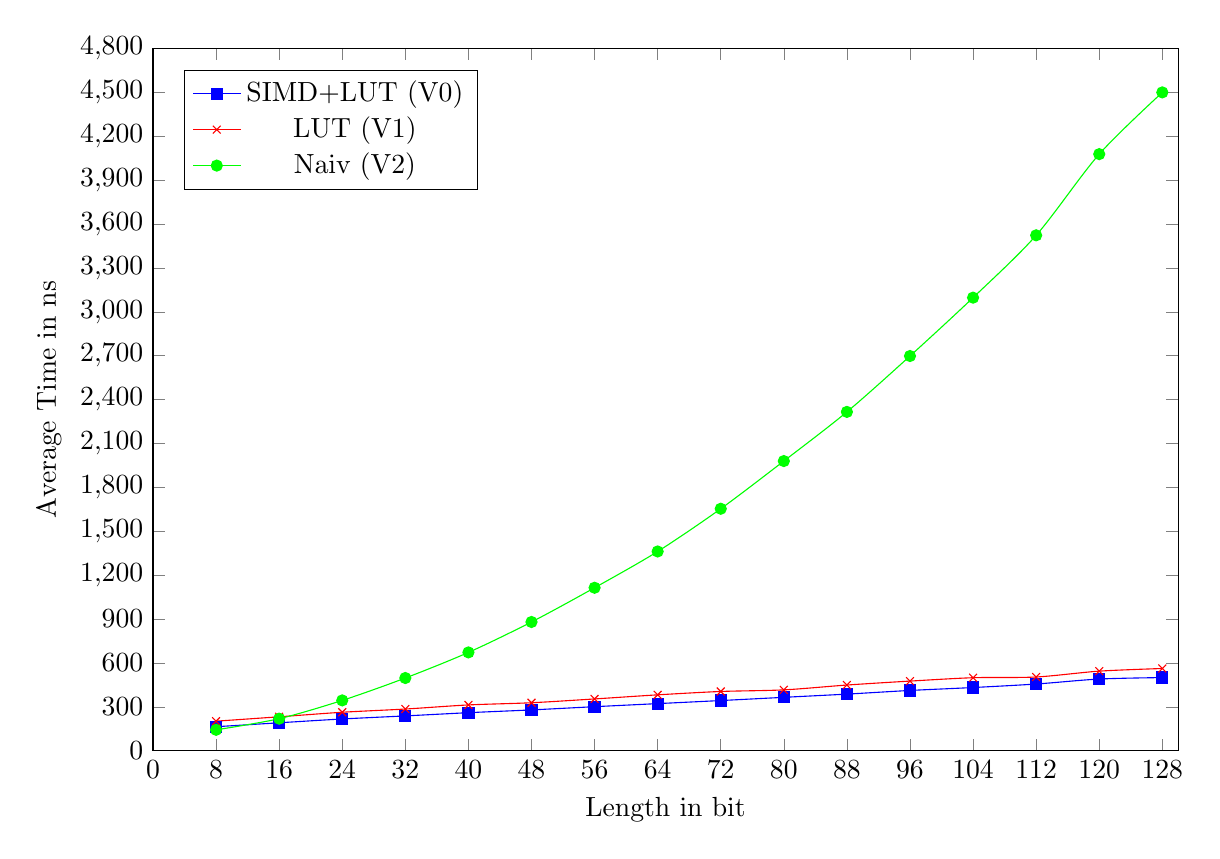
\begin{tikzpicture}
    \begin{axis}[
        width=14.6cm,
        height=10.5cm,
        xlabel=Length in bit,
        ylabel=Average Time in ns,
        xmin=0, xmax=130,
        ymin=0, ymax=4800,
        % xtick={8, 16, 24, 32, 40, 48, 56, 64},
        xtick distance=8,
        ytick distance=300,
        legend pos=north west
        ]
    \addplot[smooth,mark=square*,blue] plot coordinates {
        (8,164)
        (16,191)
        (24,217)
        (32,238)
        (40,260)
        (48,279)
        (56,301)
        (64,322)
        (72,343)
        (80,365)
        (88,387)
        (96,412)
        (104,432)
        (112,456)
        (120,490)
        (128,500)
    };
    \addlegendentry{SIMD+LUT (V0)}



    \addplot[smooth,color=red,mark=x]
        plot coordinates {
            (8,202)
            (16,232)
            (24,263)
            (32,285)
            (40,313)
            (48,328)
            (56,354)
            (64,382)
            (72,405)
            (80,416)
            (88,449)
            (96,476)
            (104,499)
            (112,504)
            (120,544)
            (128,562)
        };
    \addlegendentry{LUT (V1)}
    
    
    
    \addplot[smooth,mark=*,green] plot coordinates {
        (8,143)
        (16,219)
        (24,344)
        (32,497)
        (40,672)
        (48,880)
        (56,1114)
        (64,1362)
        (72,1654)
        (80,1980)
        (88,2316)
        (96,2698)
        (104,3097)
        (112,3523)
        (120,4078)
        (128,4500)
    };
    \addlegendentry{Naiv (V2)}
    \end{axis}
\end{tikzpicture}
}
\end{figure}

\noindent
% \begin{itemize}
% \item
\textbf{LUT und SIMD Optimierung}
Aus dem Graphen geht hervor, dass die Hauptimplementierung(SIMD+LUT) die schnellste ist und eine lineare Laufzeit mit zunehmender Bitlänge der Eingabe aufweist. Die reine LUT-Implementierung zeigt einen leichten Anstiegstrend, was auf eine lineare Zeitkomplexität hinweist. Der Anstieg ist nahezu identisch mit der Hauptimplementierung, jedoch ist die Laufzeit im Allgemeinen etwas langsamer. In beiden Fällen wird hauptsächlich eine For-Schleife mit 126 Iterationen ausgeführt. In jeder Iteration werden einige konstante Operationen wie logische UND-, Bit-Shift- und Vergleichsoperationen mit 0 durchgeführt. Zusätzlich gibt es Additions- und Load-Operationen, wenn das entsprechende Bit gesetzt ist. Je länger die Zahl, desto mehr Bits werden gesetzt. Beide Algorithmen haben eine lineare Laufzeitkomplexität:
$$V0: O(a_0 \cdot n + c \cdot 126)=O(a_0 \cdot n),\hspace{0.5em}V1: O(a_1 \cdot n + c \cdot 126)=O(a_1  \cdot n),\hspace{0.5em}a_0<a_1$$
wobei $c$ die Zeit für die Operationen entspricht, die in jeder Iteration ausgeführt werden müssen, und $a_0$ und $a_1$ die Zeit für die Operationen, wenn das entsprechende Bit gesetzt ist. $n$ ist der Anzahl der gesetzten Bits. Die letzten Iterationen werden speziell behandelt.\\
Ursprünglich hatten wir eine Beschleunigung von 2x durch die SIMD-Optimierung im Vergleich zur reinen LUT-Implementierung erwartet, da wir die beiden Additionen von Real- und Imaginärteil mit der \texttt{\_mm\_add\_epi64}-Instruktion auf eine Addition reduziert hatten. Allerdings muss immer noch in jeder Iteration der Offset zusätzlich mit einer Addition berechnet werden, was insgesamt ebenfall\textbf{}s 2 Additionen entspricht. Mit der Verwendung von \texttt{\_mm\_loadu\_si128} haben wir jedoch immer noch eine Load-Operation weniger in jeder Iteration im Vergleich zur reinen LUT-Implementierung. Dies ist auch der Grund ist, warum $a_0 < a_1$. Bei der reinen LUT-Implementierung müssen Real- und Imaginärteil separat mit Array-Zugriffen geladen werden, was zu einer etwas längeren Laufzeit bei jeder Bitlänge führt. \\
% \item
\textbf{Naive Implementierung} Die Ausführungszeit der naiven Implementierung steigt mit der steigenden Bitlänge quadratisch an. In der Hauptschleife werden auch einige Grundoperationen durchgeführt, und wenn das Bit gesetzt ist, werden zusätzlich 2 Additionen und die Funktion \texttt{exponent\_of\_base} aufgerufen, die $(-1+i)^n$ berechnet. Die Funktion \texttt{exponent\_of\_base} selbst führt hauptsächlich eine For-Schleife aus, die eine lineare Laufzeit hat. Daher liegt die Laufzeit der V2 am Ende in der Komplexitätsklasse:
$$O(128 \cdot c + \sum_{n\in I} n) = O(n^2), \hspace{0.5em}I\subseteq \{0, 1, 2, ..., 127\}$$
was einer quadratischen Komplexität entspricht. $I$ ist die Menge der Indizes der gesetzten Bits und $c$ ist die Zeit für die Operationen in jeder Iteration.
\subsection{to\_bm1pi}
Analog zu \texttt{to\_carthesian}, haben wir zufällige komplexe Zahlen als Eingabe generiert, deren binäre Darstellung Bitlängen zwischen 8 und 128 sind, ebenso mit einem Abstand von 8. Die Anzahl der Ausführungsiterationen bleibt ebenfalls konstant bei 1.000.000. 

% \begin{itemize}
    % \item
    \noindent
    Die Laufzeit beider Implementierungen steigt mit zunehmender Bitlänge linear an, wobei V1 eine etwas größere Steigung aufweist im Vergleich zu V0. V0 verwendet eine Multi-Division-Optimierung, die mit steigender Bitlänge allmählich mehr Zeit einspart. Beide Implementierungen führen hauptsächlich eine \texttt{while}-Schleife durch, in der nur die vier Grundrechenarten durchgeführt werden. Daher liegen V0 und V1 beide in der lineare Laufzeitklasse:
    $$O(a \cdot n),\hspace{0.5em}O(b \cdot n)\hspace{0.5em}mit\hspace{0.5em}a>b$$

    \noindent
    wobei $a$ und $b$ die Zeit für die eigentliche Berechnung repräsentieren und $n$ die Bitlänge der binären Darstellung der komplexen Zahl beschreibt. Das Ergebnis wird im folgenden Diagramm dargestellt:\\
    \begin{figure}[H]
\centering
\scalebox{0.9}{
\centering
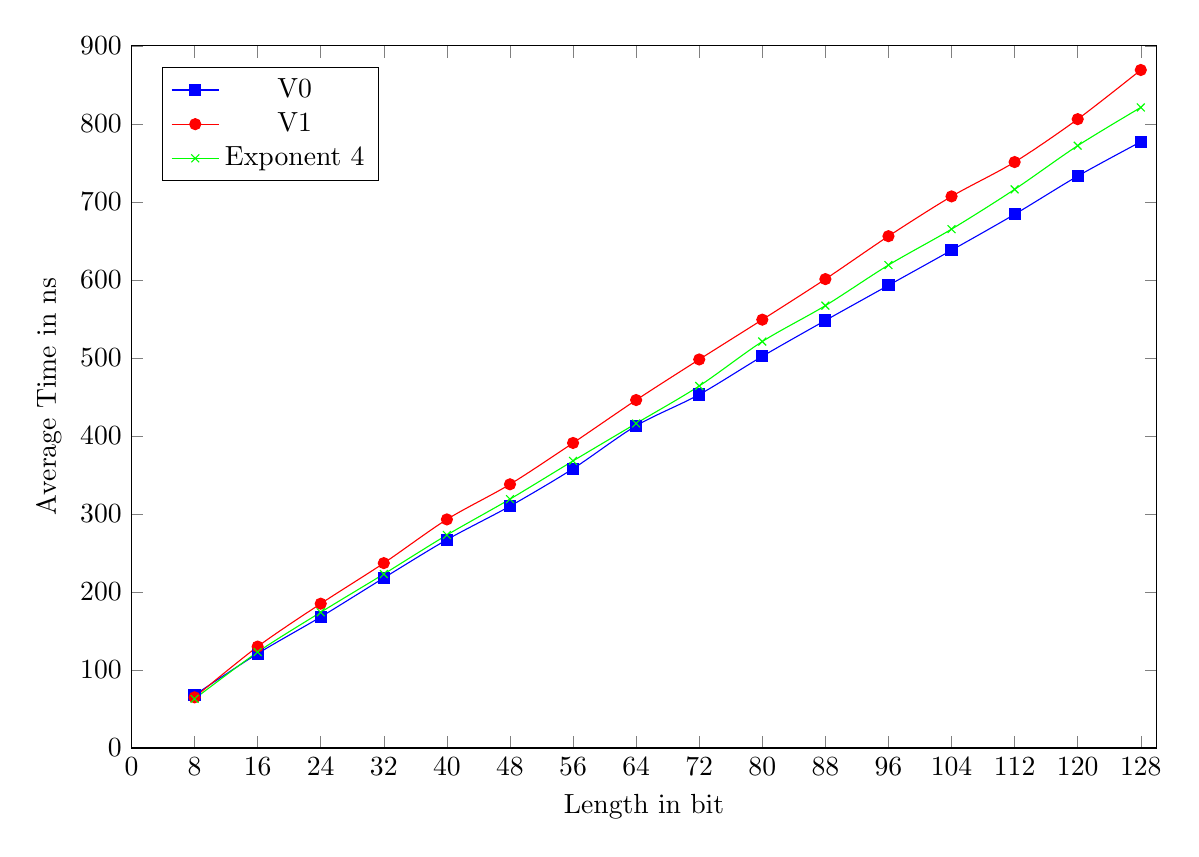
\begin{tikzpicture}
    \begin{axis}[
        width=14.6cm,
        height=10.5cm,
        xlabel=Length in bit,
        ylabel=Average Time in ns,
        xmin=0, xmax=130,
        ymin=0, ymax=900,
        % xtick={8, 16, 24, 32, 40, 48, 56, 64},
        xtick distance=8,
        ytick distance=100,
        legend pos=north west
        ]
    \addplot[smooth,mark=square*,blue] plot coordinates {
            (8,68)
            (16,121)
            (24,168)
            (32,218)
            (40,267)
            (48,310)
            (56,358)
            (64,413)
            (72,453)
            (80,502)
            (88,548)
            (96,593)
            (104,638)
            (112,684)
            (120,733)
            (128,777)
    };
    \addlegendentry{V0}
    
    \addplot[smooth,mark=*,red] plot coordinates {
            (8,65)
            (16,130)
            (24,185)
            (32,237)
            (40,293)
            (48,338)
            (56,391)
            (64,446)
            (72,498)
            (80,549)
            (88,601)
            (96,656)
            (104,707)
            (112,751)
            (120,806)
            (128,869)
    };
    \addlegendentry{V1}

    \addplot[smooth,mark=x,green] plot coordinates {
            (8,63)
            (16,123)
            (24,174)
            (32,223)
            (40,273)
            (48,319)
            (56,368)
            (64,416)
            (72,464)
            (80,521)
            (88,567)
            (96,619)
            (104,665)
            (112,716)
            (120,772)
            (128,821)
    };
    \addlegendentry{Exponent 4}
    
    
    \end{axis}
\end{tikzpicture}
}
\end{figure}
\noindent
    Die Optimierung zielt darauf ab, die Berechnung für aufeinanderfolgende 0en zu überspringen bzw. nur einmal durchzuführen, wenn die Zahl durch $(-1+i)^2$ oder $(-1+i)^3$ ohne Rest teilbar ist. Je länger die Bitlänge der binären Darstellung der komplexen Zahl, desto mehr aufeinanderfolgende Blöcke von Nullen es gibt. Daher spart V0 mit zunehmender Bitlänge allmählich mehr Zeit. Wir haben die Exponenten 2 und 3 von $(-1+i)$ gewählt, da sie die wahrscheinlichsten Längen für aufeinanderfolgende Blöcke von Nullen sind. Größere Exponenten könnten theoretisch auch verwendet werden, was jedoch zu mehr Modulo- und Vergleichsoperationen führen würde und die Gesamtlaufzeit verlangsamen würde, wie im Diagramm dargestellt.
    % \item 
    Die folgende Tablle zeigt 2 F{\"a}lle, wobei unsere Optimierung besonders gut und sogar langsamer ist:
    
    \begin{center}
    \begin{tabular}{||c|c|c|c|c||}
    \hline
    real & imag & time(V0) & time(V1) & bm1pi\\
    \hline
    4096 & 0  & 63ns & 139ns & 1000000000000000000000000\\
    \hline
    -1638 & -819  & 162ns  & 155ns & 111111111111111111111111\\
    \hline
    \end{tabular}
\end{center}
Im ersten Fall hat die zu konvertierende komplexe Zahl $4096 + 0i$ eine binäre Darstellung, bei der nur das signifikante Bit 1 ist und alle anderen Bits 0 sind. Dabei überspringt V0 die sukzessiven Nullen sehr schnell und weist im Vergleich zur naiven Implementierung eine Beschleunigung von mehr als 2x auf.\\
Im zweiten Fall gibt es keine aufeinanderfolgenden Nullen, daher ist V0 sogar langsamer, da in jeder Iteration zusätzlich zwei \texttt{if}-Konditionen überprüft werden müssen.
\subsubsection{Einfluss des Caches auf die Leistung}
Der Cache spielt eine wichtige Rolle, insbesondere wenn das Programm mit der Option \texttt{-B} und einer großen Anzahl an Iterationen ausgeführt wird. Die durchschnittliche Laufzeit kann sich erheblich unterscheiden, aufgrund der unterschiedlichen Anzahl von Cache-Misses.
Als Beispiel: Bei der Ausführung des Befehls \texttt{./cbns 52045582664164951 -B1000000}, wobei 52045582664164951 eine 32-Bit-lange Zahl ist, kann der Cache einen signifikanten Einfluss auf die Laufzeit haben.
    \begin{center}
    \begin{tabular}{||c|c|c||}
    \hline
    Eingabe & Cache-Misses & Zeit\\
    \hline
    52045582664164951 & 6   & 135ns\\
    \hline
    zuf{\"a}lligen 56-bit Zahlen & 340  & 303ns\\
    \hline
    \end{tabular}
\end{center}
Im ersten Fall werden die Daten, die von der LUT (Lookup-Tabelle) geladen wurden, im Cache gespeichert und in den nächsten Iterationen wiederverwendet, da die Eingabe unverändert bleibt. Im Gegensatz dazu ist die Wahrscheinlichkeit der Wiederverwendung im Fall zufälliger Eingaben deutlich geringer. Dies liegt daran, dass die Indizes der gesetzten Bits jedes Mal unterschiedlich sind, was zu einer erhöhten Anzahl von Cache-Misses führt. Bei der Funktion \texttt{to\_bm1pi()} besteht eine ähnliche Situation.

\section{Zusammenfassung und Ausblick}
Unsere allgemeine Vorgehensweise lässt sich wie folgt beschreiben: Zuerst implementieren wir eine naive L{\"o}sung, dann versuchen wir, die einzelnen Rechenschritte zu parallelisieren.\\
Genauer betrachtet haben wir in \texttt{void to\_carthesian} zuerst versucht, durch die Bitstellen zu iterieren und die entsprechende Potenz von$-1 + i$ zu berechnen. Dieses Zwischenergebnis haben wir dann zum Endergebnis addiert. Zur Optimierung haben wir die Potenzen von $-1 + i$ bis zu 128 Stellen im Voraus berechnet und in eine Lookup-Tabelle eingetragen. Dadurch konnten wir teure Multiplikationen vermeiden, indem wir nicht jedes Mal die Potenz berechnen mussten. Am Ende haben wir auch 128-Bit-SSE-Register verwendet, um den Real- und Imaginärteil gleichzeitig zu laden. Dies ermöglicht es uns, bis auf zwei Real- oder Imaginärteile, die nicht mehr in einem 64-Bit-Register passen, effizient zu verarbeiten. Dadurch sparen wir einen Ladeschritt.\\
In \texttt{unsigned \_\_int128 to\_bm1pi} haben wir zuerst versucht, analog zu den üblichen Basiskonvertierungen, die komplexe Zahl Schritt für Schritt durch $-1 + i$ zu dividieren, bis es keinen Rest mehr gibt. Zur Optimierung haben wir die Zahl in jedem Schritt durch die mehrfach Potenz von $-1 + i$ dividiert, um unnötige Divisionsschritte zu sparen.\\
Eine weitere Vorgehensweise\cite{CBNS} ist die Konvertierung kartesischer Zahlen in Basis -4 und anschlie{\ss}endes Konvertieren in Basis $(-1 + i)$. Diese Methode braucht, dass man auch Arithmetik in Basis $(-1 + i)$ implementiert, und daher auch Rechnen mit $(-1 + i)$ Basis Bitstrings erm{\"o}glicht. Diese ist allerdings von uns nicht implementiert und nur als Ausblick erw{\"a}hnt.


% TODO: Fuegen Sie Ihre Quellen der Datei Ausarbeitung.bib hinzu
% Referenzieren Sie diese dann mit \cite{}.
% Beispiel: CR2 ist ein Register der x86-Architektur~\cite{intel2017man}.

\newpage

\bibliographystyle{plain}
\bibliography{Ausarbeitung}{}

\end{document}
